%\section{Démarche méthodologique}
%La partie précédente a mis en évidence que différentes méthodes pouvaient être mobilisées pour %traiter les données issues du réseau social en ligne Twitter. Comme pour la majorité des %recherches s’appuyant sur cette source de données particulière, plusieurs méthodes sont ici %mobilisées successivement. Nous détaillons tout d’abord les modalités de collecte et de %construction de la base de données. Nous présentons ensuite les différentes méthodes d’analyse %utilisées.
%
%\subsection{Création de la base de données}
%
%La collecte des données s’est faite en plusieurs étapes.
%\begin{itemize}
%    \item Dans un premier temps, une liste de comptes d’organisations a été constituée.
%    \item Dans un second temps, les tweets publiés par ces organisations ainsi que des données %complémentaires ont été téléchargés et enregistrés dans une base de données.
%\end{itemize}
%
%\subsubsection{Constitution de la liste des comptes Twitter}
%Pour mettre en place l’échantillon étudié, un compte Twitter spécialement dédié à cette recherche %a été créé. Les utilisateurs intégrés à l’échantillon sont matérialisés par les abonnements de ce %compte dédié.
%
%Deux méthodes sont utilisées conjointement pour constituer la liste.
%
%Dans un premier temps, des entreprises de l’ESS sont identifiées à partir de sources %institutionnelles. Lorsqu’elles possèdent un compte Twitter, celui-ci est ajouté aux abonnements. %Les listes mobilisées proviennent du CNCRES, de l’ACP ou de la base ‘open data’ du gouvernement :
%\begin{itemize}
%    \item Liste des 100 principales coopératives (CNCRES)
%    \item Liste des sociétés commerciales de l’ESS (\url{http://liste-entreprises.cncres.org/})
%    \item Liste des associations reconnues d’utilité publique (data.gouv)
%    \item Liste des fondations reconnues d’utilité publique (data.gouv)
%    \item Liste des mutuelles (ACP)
%\end{itemize}
%
%Pour les deux premières, l’ensemble des entreprises a été traité ; pour les trois suivantes, étant %donné le nombre considérable d’entreprises, une sélection aléatoire a été effectuée. Cette %première approche nous garantit l’intégration d’une grande variété d’entreprises à l’échantillon.
%
%La seconde approche se fait directement dans l’interface web de twitter, et s’appuie sur des %recherches et suggestions. Une recherche sur des mots clés renvoyant aux \eess (‘coopérative’, %‘socent’, ‘association’, etc.) a permis d’identifier les comptes d’entreprises de l’ESS ayant la %meilleure visibilité. Les comptes pertinents pour la recherche ont été ajoutés aux abonnements. %L’algorithme de Twitter propose des suggestions de comptes en lien avec les utilisateurs auxquels %le compte est déjà abonné. Ces comptes suggérés sont étudiés au cas par cas afin de déterminer %s’ils peuvent être ajoutés au panel. Cette méthode est répétée de manière itérative (les %suggestions étant actualisées à chaque nouvel abonnement), et permet un effet « boule de neige ». %Une limite notable de cette méthode est qu’elle fonctionne « en circuit fermé » : elle permet %d’identifier uniquement des comptes connectés entre eux. Toutefois, la sélection aléatoire %réalisée dans l’étape 1 garantie une certaine ouverture dans ces suggestions.
%
%\paragraph{Critères d'intégration à la liste.}
%
%Le choix d’intégrer un compte à la liste est fait en se basant sur la description de %l’utilisateur, ou le cas échéant, sur le site internet de l’entreprise. Les comptes ajoutés à la %liste sont les suivants :
%\begin{itemize}
%    \item Comptes d’entreprise de l’ESS (association, coopérative, mutuelle, association, %fondation, entreprise sociale, entreprise d’insertion…),
%    \item Comptes d’organismes de représentation de l’ESS (CRESS, CGSCOP…),
%    \item Comptes d’incubateurs d’entreprises dédiés à l’ESS,
%    \item Comptes d’évènements liés à l’ESS (Le mois de l’ESS…),
%    \item Comptes de marques d’entreprises de l’ESS.
%\end{itemize}
%
%Les comptes individuels (militants, étudiants, enseignants, chercheurs, dirigeants ou employés de %l’ESS, responsables politiques en charge de l’ESS) et les comptes des médias dédiés à l’ESS ne %sont pas intégrés à la liste. Ce choix est fait afin de centrer le corpus sur le discours en %provenance des acteurs de l’ESS, et non de personnes intéressées par ce secteur ou ayant une %posture critique.
%
%Seuls ont été pris en compte les utilisateurs dont la description et les messages sont en langue %française (essentiellement des entreprises françaises, mais également belges et québécoises).
%
%Dans la mesure où certains comptes (toutefois minoritaires) ne correspondent pas à des %entreprises, on parlera pour cette étude « d’organisations »\footnote{Dans le reste de la thèse, %on s’alignera sur la perspective adoptée par le CNCRES, et on parlera d’entreprises de l’ESS %(EESS).}.
%

%
%Le tableau \ref{table:2} résume les données rattachées à chaque utilisateur. La majorité est %directement issue de Twitter. Toutefois, le type d’organisation correspondant à un compte et la %dimension environnementale ou non de son activité sont ajoutés manuellement de la façon décrite %ci-dessous.
%
%Les organisations sont affectées à l’une des catégories suivantes : Association, Coopérative (dont %SCP, SCIC, SCE, coopératives d’entreprises, coopératives d’usagers, coopératives bancaires, autres %coopératives) Fondation, Fédération, Mutuelle, Incubateur, Entreprise sociale, Autre. Il faut %souligner que cette répartition ne repose pas strictement sur la forme juridique des entreprises, %mais davantage sur la présentation des entreprises. Ainsi, alors qu’on ne recense que 93 sociétés %commerciales dans l’ESS fin 2016 \parencite{atlas2017}, l’échantillon comprends près de 72 « %entreprises sociales ». En réalité, de nombreuses entreprises adoptent un statut associatif ou %coopératif, mais se définissent comme entreprise sociale. Au-delà du statut, ceci traduit une %volonté de s’inscrire dans un courant et dans une démarche particulière. Pour cette raison, les %associations, fondations ou coopératives qui se présentent explicitement comme des entreprises %sociales dans leur description sont affectées à la catégorie « entreprises sociales ». De mêmes la %catégorie « Fédération » ne constitue pas une forme juridique d’entreprise. Ce groupe est %constitué de tous types d’entreprises qui ont pour spécificité de rassembler et de fédérer un %réseau d’organisations. La catégorie « autre » regroupe des comptes qui ne sont pas des comptes %d’entreprises, mais des comptes correspondants à des marques, évènements ponctuels ou réseaux %informels. Ainsi, la catégorisation réalisée ici n’a pas pour vocation à reproduire la répartition %de l’ESS en différents statuts, mais plutôt à apporter des éléments d’analyse.
%
%La détermination de la dimension environnementale nécessite une analyse plus fine de %l’organisation. Les critères suivants sont appliqués :
%\begin{itemize}
%    \item	Si l’organisation a une activité principale directement liée à l’environnement, elle %est qualifiée d’organisation environnementale (OE) : la variable prend la valeur VRAIE.
%    \item	Si l’organisation a une activité principale non liée à l’environnement, la variable %prend la valeur FAUX.
%    \item	Si l’organisation a une activité principale indirectement liée à l’environnement, la %valeur est VRAI uniquement si la dimension écologique est mise en avant dans la description du %compte. Par exemple, une épicerie bio est considérée comme environnementale uniquement si elle %indique que la démarche bio est adoptée pour des raisons écologiques. De même, une association %de protection des animaux est considérée comme environnementale si la finalité est la %préservation de l’écosystème.
%\end{itemize}
%
%
%
%\subsubsection{Collecte, enregistrement et préparation des données}
%
%En raison du volume des données, la collecte ne peut être faite via l’interface web et nécessite %l’usage de programmes spécifiques. Une solution fréquemment retenue est l’utilisation du langage %informatique Python qui permet d’interroger directement l’interface développeur (API) de Twitter. %Plusieurs scripts Python ont ainsi été écrits afin de collecter les tweets, les enregistrer et %retraiter le contenu pour permettre l’analyse (voir annexes).
%
%Twitter limite le nombre de tweets collectés à 200 par utilisateur et par requête. Par conséquent, %un processus itératif a été déployé afin de collecter le plus grand nombre possible de tweets pour %chaque utilisateur du panel. Les tweets les plus récents sont collectés en priorité. La recherche %se limite aux tweets originaux (c'est-à-dire que les retweets sont exclus) et en français. %Toutefois, l’information de la langue est parfois incorrecte dans la base Twitter et certains %tweets dans d’autres langues peuvent donc être collectés.  Les données collectées pour chaque %tweet sont synthétisées dans le tableau \ref{table:3tweets}.
%
%\begin{table}
%    \caption{Données relatives aux tweets}
%    \label{table:3tweets}
%        \begin{tabularx}{\linewidth}{|L|L|}
%            \hline
%            \textbf{Nom} & \textbf{Description} \\ \hline
%            Id tweet&	Numéro unique d’identification du tweet \\ \hline
%            Nom utilisateur&	Nom de l’utilisateur ayant posté le tweet \\ \hline
%            Id utilisateur&	Identifiant de l’utilisateur ayant posté le tweet \\ \hline
%            Date&	Date exacte de publication du tweet au format AAAA-MM-JJ hh:mm:ss.000000 \\ %\hline
%            Année&	Année de publication du tweet (format AAAA) \\ \hline
%            Mois&	Mois de publication du tweet (format MM) \\ \hline
%            Texte&	Texte complet du tweet \\ \hline
%            Hashtags&	Mots clés utilisés dans le message (précédés de ‘\#’) \\ \hline
%            Nombre favoris*	&Nombre de fois où le tweet a été mis en favori \\ \hline
%            Nombre retweets*&	Nombre de fois où le tweet a été partagé \\ \hline
%            Id mentions	&Identifiant numérique des utilisateurs mentionnés dans le tweet \\ \hline
%            Nom mentions&	Nom des utilisateurs mentionnés dans le tweet \\ \hline
%             \multicolumn{2}{K{0.95\linewidth}}{\footnotesize{*Ces données sont susceptibles %d’évoluer dans le temps. Elles ne sont donc pas représentatives pour les tweets %récents et ont donc été mise à jour un mois après la fin de la collecte pour garantir %une certaine fiabilité.}}
%        \end{tabularx}
%\end{table}
%
%Les données collectées sont stockées dans une base de données au format SQLite. Toutes les %opérations effectuées sur la base de données sont effectuées via des scripts Python, et sont ainsi %documentées précisément (voir annexes).
%
%\paragraph{Détermination du caractère environnemental d’un tweet.} Une partie de l’étude %s'intéresse uniquement aux tweets qui traitent de questions environnementales. Il est donc %nécessaire de déterminer des critères permettant d’éliminer les tweets n’ayant aucun lien avec %cette thématique. Trois critères sont utilisés.
%\begin{itemize}
%    \item Le premier critère retient tous les tweets évoquant directement « l’environnement » ou « %l’écologie ». Il s’agit des contenus comportant un mot ayant la racine ‘environn’ ou ‘écolo’.
%    \item Le second critère est plus ouvert. Parmi les 3000 hashtags les plus couramment utilisés %dans le corpus de tweets, 101 hashtags relatifs à la question environnementale ont été %identifiés (cf. encadré \ref{encadre:1}). Tous les tweets utilisant un de ces hashtags sont %retenus.
%    \item Le critère 3 retient tous les tweets ayant un caractère environnemental selon l’un des %deux critères précédents. C’est le critère qui est retenu pour l’ensemble de l’étude.
%
%\end{itemize}
%
%\begin{encadre}
%    \caption{Principaux hashtags relatifs à l'environnement}
%    \label{encadre:1}
%    \fbox{
%    \begin{minipage}{\linewidth}
%        \footnotesize
%        accorddeparis, agroecologie, agroécologie, antigaspi, ateliercoecolo, bio, biocentrisme, %biodéchets, biodiversite, biodiversité, changementclimatique, changerclimats, charbon, %circuitcourt, circuitscourts, climat, climatdatalab, climatechange, climatgeopolble, %climatique, confenvi, cop21, cop21paris, dd, déchet, dechets, déchets, deforestation, %déforestation, devdurable, developpementdurable, développementdurable, durable, eco, %ecocollab, écolo, ecologie, écologie, écologique, economiecirculaire, économiecirculaire, %emballages, énergétique, energie, énergie, energiecitoyenne, énergies, %energiesrenouvelables, environment, environnement, environnementale, éolien, foret, forêt, %forêts, gazdeschiste, gocop21, greenwashing, huiledepalme, loibiodiv, loup, loups, nature, %naturealert, nucleaire, nucléaire, obsolescenceprogrammée, oceanclimax, ogm, ouiauxloups, %pêcheprofonde, permaculture, pesticides, petitionpesticides, pétrole, photovoltaique, %photovoltaïque, plantfortheplanet, pollution, pollutionair, pollutiondelair, %projectrescueocean, recyclage, recycler, recyclivredays, réemploi, renouvelable, %renouvelables, rénovationénergétique, sosloups, stopcharbon, stopdeforestation, %stoppesticides, transitionecologique, transitionenergetique, transitionenergétique, %transitionénergétique, zerodechet, zérodéchet, zérodéforestation, zerowaste
%        \end{minipage}
%        }
%\end{encadre}
%
%
%L’utilisation de ces critères conduit à réduire considérablement le nombre de tweets étudiés. En %effet, parmi l’ensemble des contenus publiés par les utilisateurs de l’ESS, seule une faible %proportion concerne l’environnement. Ceci s’explique d’une part par le fait que seule une minorité %d’\eess a une mission environnementale, et d’autre part parce que toutes sont confrontées à des %sujets très variés. L’environnement ne constitue donc qu’une partie de leur discours. C’est %toutefois ce contenu réduit qui intéresse l’étude. On peut dès lors s’interroger sur la pertinence %de collecter une telle masse de données (près d’un million de tweets) pour finalement n’en garder %qu’une faible proportion. Cependant, la nature de la source de données (Twitter) fait qu’il est %plus simple de collecter un ensemble de données très large et de le réduire ensuite. Ainsi, pour %des études similaires, \textcite{kwon2015spatiotemporal} ne codent que 5\% des données collectées, %\textcite{stefanone2015image} analysent 290 images collectées parmi 15840 tweets et %\textcite{xu2014twitter} limitent leur analyse à 3319 tweets sur 125907 collectés. La section %suivante synthétise les volumes collectés et analysés pour la présente étude.
%
%
%
%\subsubsection{Synthèse des données collectées}
%L’échantillon final est constitué de 1110 comptes d’utilisateurs répartis en 8 catégories. Le %tableau \ref{table:4categories} détaille cette répartition, et le tableau \ref{table:5coop} %précise la ventilation en différents statuts coopératifs. Les associations représentent près de la %moitié des organisations de l’échantillon. Ceci s’explique par la très forte prépondérance de ce %statut dans l’\ess où les associations représentent 93.9\% des entreprises et 77.7\% de l’emploi %\parencite{atlas2017}. La relative sous-représentation des mutuelles dans l’échantillon s’explique %par leur faible présence sur Twitter. La majorité des comptes de mutuelles correspondent à des %fédérations (telles que la Mutualité Française).
%
%
%\begin{table}
%\begin{footnotesize}
%\noindent
%\begin{minipage}{0.35\textwidth}
%\centering
%    \caption{Catégories d'utilisateurs}
%    \label{table:4categories}
%        \begin{tabularx}{\textwidth}{|L|R|}
%
%            \hline
%            \head{Catégorie} & \finalhead{Nombre d'utilisateurs} \\ \hline
%            Association	&544\\ \hline
%            Coopérative&	191\\ \hline
%            Fondation&	114\\ \hline
%            Fédération&	111\\ \hline
%            Entreprise sociale&	73\\ \hline
%            Mutuelle&	50\\ \hline
%            Autre&	27\\ \hline
%            \textbf{Total}	& \textbf{1110} \\ \hline
%        \end{tabularx}
%\end{minipage}
%\hspace{0.5cm}
%\begin{minipage}{0.58\linewidth}
%\centering
%\caption{Types de coopératives}
%\label{table:5coop}
%    \begin{tabularx}{\linewidth}{|K{0.60\linewidth}|R|}
%
%        \hline
%        \head{Catégorie} & \finalhead{Nombre d'utilisateurs} \\ \hline
%        Sociétés coopératives et participatives (SCOP et CAE)&	75\\ \hline
%        Coopérative d’entreprises&	49\\ \hline
%        SCIC&	39\\ \hline
%        Coopérative bancaire&	20\\ \hline
%        Coopérative d’usagers&	6\\ \hline
%        Autres coopératives&	1\\ \hline
%        Sociétés coopératives européennes (SCE)	&1\\ \hline
%
%        \textbf{Total coopératives}	& \textbf{191} \\
%        \hline
%    \end{tabularx}
%
%\end{minipage}
%\end{footnotesize}
%\end{table}
%
%Au total, 910 649 tweets originaux sont collectés, sur une période allant du mois d’août 2008 à %fin juin 2017. Comme le montre la figure \ref{figure:1}, le nombre de tweet augmente fortement %d’année en année, et la majorité des tweets se concentre sur la période récente (2012 à 2017).
%
%\begin{figure}
%    \caption{Nombre de tweets collectées par années}
%    \label{figure:1}
%    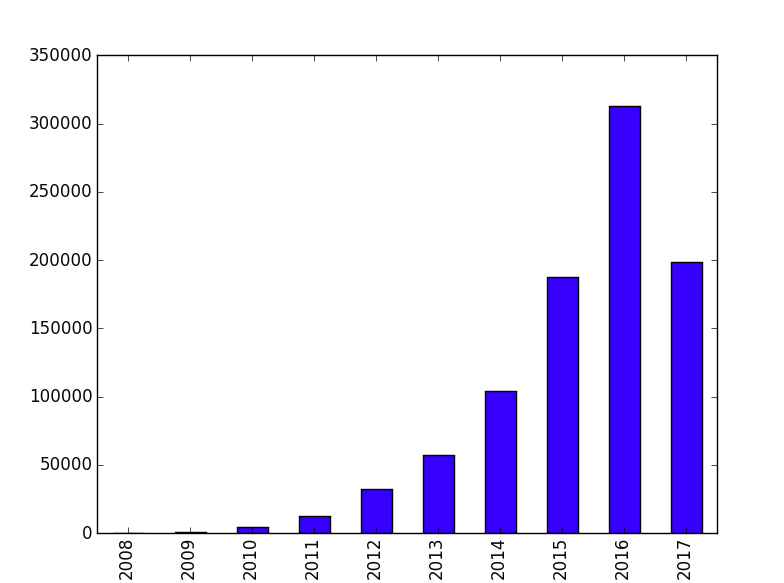
\includegraphics[width=10cm]{fig/fig1.png}
%
%\end{figure}
%
%
%\subsection{Analyse statistique}
%
%Plusieurs méthodes statistiques sont mobilisées afin d’analyser les données. Elles sont mises en %œuvre à l’aide de Python. Des statistiques descriptives sont mobilisées pour mettre en évidence %les modalités d’utilisation du réseau social. Les liens entre différentes variables sont testés à %l’aide de régressions multiples. Enfin, des tests non paramétriques sont utilisés pour comparer %différentes catégories de comptes (type d’entreprise, mission environnementale ou non). Le recours %à ce type de tests est imposé par la structure des données, qui ne respectent pas les conditions %d’application de tests paramétriques.
%
%\subsection{Analyse lexicale}
%Cette phase de l’étude s’intéresse plus précisément au sens des messages diffusés sur le réseau. %L’analyse lexicale permet d’étudier isolément les mots du corpus, c'est-à-dire détachés de leur %contexte. L’analyse repose sur la quantification des formes lexicales. L’étude s’appuie %spécifiquement sur les hashtags, c'est-à-dire les éléments du tweet mis en avant par l’émetteur du %message. Ce procédé n’est pas obligatoire, mais est mobilisé pour une proportion importante de %tweets (47.3\% du total des tweets collectés). L’étude utilise les hashtags pour déterminer le %cadre rhétorique dans lequel s’inscrit un message. Les cadres renvoient à la façon dont le %discours donne du sens à son objet. Comme le souligne \textcite{nisbet2009communicating}, toute %information s’inscrit dans un cadre donné. Il identifie huit cadres utilisés dans la communication %sur le changement climatique, qui peuvent s’appliquer à l’ensemble des enjeux écologiques. Le  %tableau \ref{table:6} présente ces cadres et précise les modalités d’opérationnalisation.
%
%
%
%\begin{landscape}
%\begin{spacing}{1}
%\begin{small}
%    \begin{longtable}{|K{0.18\linewidth}|K{0.38\linewidth}|K{0.40\linewidth}|}
%        \caption{Typologie des cadres du discours}
%        \label{table:6} \\
%            \hline
%            \textbf{Cadre} & \textbf{Définition \parencite{nisbet2009communicating} \newline %Frames define science-related issue as…} & \textbf{Opérationnalisation}\\ \hline
%            \endfirsthead
%            \hline
%            \textbf{Cadre} & \textbf{Définition \parencite{nisbet2009communicating}} & %\textbf{Opérationnalisation}\\ \hline
%            \endhead
%            \hline
%                Progrès Social
%                &A means of improving quality of life or solving problems; alternative %interpretation as a way to be in harmony with nature instead of mastering it.
%                &Le cadre est élargi aux hashtags qui renvoient à des questions d’ordre sociétal
%                \\ \hline
%
%                Développement économique et compétitivité
%                &An economic investment; market benefit or risk; or a point of local, national, or %global competitiveness.
%                &Le cadre intègre tous les hashtags qui renvoient à des dimensions d’économie, %d’emploi, de compétitivité ou à la notion de marché
%                \\ \hline
%
%                Moralité et éthique
%                &A matter of right or wrong; or of respect or disrespect for limits, thresholds, %or boundaries.
%                &Le cadre intègre tous les hashtags renvoyant à la morale, à des valeurs sociales, %de respect ou de solidarité.
%                \\ \hline
%
%                Incertitude scientifique et technique
%                &A matter of expert understanding or consensus; a debate over what is known versus %unknown; or peer-reviewed, confirmed knowledge versus hype or alarmism.
%                &Hashtags renvoyant plus généralement à de questions techniques et scientifiques, %sans prise de position explicite
%                \\ \hline
%
%                Boîte de Pandore, Monstre de Frankenstein et ‘Sauve-qui-peut’
%                &A need for precaution or action in face of possible catastrophe and %out-of-control consequences; or alternatively as fatalism, where there is no way %to avoid the consequences or chosen path.
%                &Hashtags renvoyant à une dimension dramatique, focalisé sur les dangers et les %risques liés à la non prise en compte de l’environnement, ainsi que les %conséquences déjà observés
%                \\ \hline
%
%                Responsabilité publique et gouvernance
%                &Research or policy either in the public interest or serving special interests, %emphasizing issues of control, transparency, participation, responsiveness, or %ownership; or debate over proper use of science and expertise in decisionmaking %(“politicization”).
%                &Hashtags renvoyant à la gouvernance aussi bien au niveau des entreprises que des %institutions publiques, ainsi que les hashtags renvoyant à une responsabilité %partagée, citoyenne
%                \\ \hline
%
%                Alternatives et compromis
%                &A third way between conflicting or polarized views or options.
%                &Hashtags renvoyant à des alternatives, des exemples d’innovations, ou plus %généralement un changement, une transition
%                \\ \hline
%
%                Conflits et stratégies
%                &A game among elites, such as who is winning or losing the debate; or a battle of %personalities or groups (usually a journalist-driven interpretation).
%                &Hashtags renvoyant à des acteurs du débat public, à des lieux d’échange et de %constitution de stratégies, ou à des prises de position claires
%                \\ \hline
%
%
%    \end{longtable}
%\end{small}
%\end{spacing}
%\end{landscape}
%
%
%
%Cette classification donne lieu à deux analyses :
%\begin{itemize}
%    \item	Une Analyse Factorielle des correspondances (AFC), qui permet de confronter les %différents modèles d’entreprises de l’ESS avec les cadres utilisés. Elle est réalisée à l’aide %du programme FactoMineR à partir d’une table de contingence créée par un script Python ;
%    \item	Des tests non paramétriques de comparaison de moyenne. Ils visent à déterminer si le %nombre de de retweets ou de favoris est significativement plus important pour certaines %catégories.
%\end{itemize}
%
%\subsection{Visualisation à l’aide des réseaux}
%
%Des données relatives aux liens entre les organisations du panel sont collectées. A l’aide du %logiciel Gephi, elles permettent d’identifier des communautés d’utilisateurs interconnectés. Le %logiciel permet également de produire des visualisations du réseau constitué par les %organisations. Celles-ci viennent compléter les résultats et montrer comment les \aess\ %s’organisent et interagissent sur le réseau social Twitter.


\section{Etude du discours sur Twitter : précisions méthodologiques}

\subsection{Constitution du panel de comptes Twitter.}

\subsubsection{Sélection des comptes d’utilisateurs}

Deux méthodes sont utilisées conjointement pour constituer la liste.

Dans un premier temps, des entreprises de l’ESS sont identifiées à partir de sources institutionnelles. Lorsqu’elles possèdent un compte Twitter, celui-ci est ajouté aux abonnements. Les listes mobilisées proviennent du CNCRES, de l’ACP ou de la base ‘open data’ du gouvernement :
\begin{itemize}
    \item Liste des 100 principales coopératives (CNCRES)
    \item Liste des sociétés commerciales de l’ESS (\url{http://liste-entreprises.cncres.org/})
    \item Liste des associations reconnues d’utilité publique (data.gouv)
    \item Liste des fondations reconnues d’utilité publique (data.gouv)
    \item Liste des mutuelles (ACP)
\end{itemize}

Pour les deux premières, l’ensemble des entreprises a été traité ; pour les trois suivantes, étant donné le nombre considérable d’entreprises, une sélection aléatoire a été effectuée. Cette première approche nous garantit l’intégration d’une grande variété d’entreprises à l’échantillon.

La seconde approche se fait directement dans l’interface web de twitter et s’appuie sur des recherches et suggestions. Une recherche sur des mots clés renvoyant aux \eess (‘coopérative’, ‘socent’, ‘association’, etc.) a permis d’identifier les comptes d’entreprises de l’ESS ayant la meilleure visibilité. Les comptes pertinents pour la recherche ont été ajoutés aux abonnements. L’algorithme de Twitter propose des suggestions de comptes en lien avec les utilisateurs auxquels le compte est déjà abonné. Ces comptes suggérés sont étudiés au cas par cas afin de déterminer s’ils peuvent être ajoutés au panel. Cette méthode est répétée de manière itérative (les suggestions étant actualisées à chaque nouvel abonnement) et permet un effet \cit{boule de neige}. Une limite notable de cette méthode est qu’elle fonctionne \cit{en circuit fermé} : elle permet d’identifier uniquement des comptes connectés entre eux. Toutefois, la sélection aléatoire réalisée dans l’étape 1 garantit une certaine ouverture dans ces suggestions.

Le choix d’intégrer un compte à la liste est fait en se basant sur la description de l’utilisateur ou, le cas échéant, sur le site internet de l’entreprise. Les comptes ajoutés à la liste sont les suivants :
\begin{itemize}
    \item Comptes d’entreprises de l’ESS (association, coopérative, mutuelle, association, fondation, entreprise sociale, entreprise d’insertion…),
    \item Comptes d’organismes de représentation de l’ESS (CRESS, CGSCOP…),
    \item Comptes d’incubateurs d’entreprises dédiés à l’ESS,
    \item Comptes d’évènements liés à l’ESS (Le mois de l’ESS…),
    \item Comptes de marques d’entreprises de l’ESS.
\end{itemize}

Les comptes individuels (militants, étudiants, enseignants, chercheurs, dirigeants ou employés de l’ESS, responsables politiques en charge de l’ESS) et les comptes des médias dédiés à l’ESS ne sont pas intégrés à la liste. Ce choix est fait afin de centrer le corpus sur le discours en provenance des acteurs de l’ESS et non de personnes intéressées par ce secteur ou ayant une posture critique.

Seuls ont été pris en compte les utilisateurs dont la description et les messages sont en langue française (essentiellement des entreprises françaises, mais également belges et québécoises).

Les données relatives aux comptes évoluent régulièrement (description, nombre d’abonnements, nombre de tweets…). Une mise à jour de tous les comptes est effectuée à l’issue de la collecte des tweets et avant la réalisation des analyses afin d’avoir les données les plus récentes.

\subsubsection{Affectation à des catégories}

Les utilisateurs sont affectés à l’une des catégories suivantes : Association, Coopérative (dont SCP, SCIC, SCE, coopératives d’entreprises, coopératives d’usagers, coopératives bancaires, autres coopératives), Fondation, Fédération, Mutuelle, Entreprise sociale, Autre. Il faut souligner que cette répartition ne repose pas strictement sur la forme juridique des entreprises, mais davantage sur la présentation des entreprises. Ainsi, alors qu’on ne recense que 93 sociétés commerciales dans l’ESS fin 2016 \parencite{observatoire_national_de_leconomie_sociale_et_solidaire_france2017atlas}, l’échantillon comprend près de 72 \cit{entreprises sociales}. En réalité, de nombreuses entreprises adoptent un statut associatif ou coopératif, mais se définissent comme entreprise sociale. Au-delà du statut, ceci traduit une volonté de s’inscrire dans un courant et dans une démarche particulière. Pour cette raison, les associations, fondations ou coopératives qui se présentent explicitement comme des entreprises sociales dans leur description sont affectées à la catégorie \cit{entreprises sociales}. De mêmes la catégorie \cit{Fédération} ne constitue pas une forme juridique d’entreprise. Ce groupe est constitué de tous types d’entreprises qui ont pour spécificité de rassembler et de fédérer un réseau d’organisations. La catégorie \cit{autre} regroupe des comptes qui ne sont pas des comptes d’entreprises, mais des comptes correspondants à des marques, évènements ponctuels ou réseaux informels. Ainsi, la catégorisation réalisée ici n’a pas pour vocation à reproduire la répartition de l’ESS en différents statuts, mais plutôt à apporter des éléments d’analyse. Le statut juridique est utilisé comme critère d’affectation en l’absence d’éléments déclaratifs. Cette information est généralement disponible dans les mentions légales du site internet de l’organisation ou sur des annuaires d’entreprises en ligne.

\subsubsection{Détermination de la dimension environnementale de l’organisation}

Elle nécessite une analyse plus fine de l’organisation. Les critères suivants sont appliqués : \begin{itemize}
    \item Si l’organisation a une activité principale directement liée à l’environnement, elle est qualifiée d’organisation environnementale (OE) : la variable prend la valeur VRAIE.
    \item Si l’organisation a une activité principale non liée à l’environnement, la variable prend la valeur FAUX.
    \item si l’organisation a une activité principale indirectement liée à l’environnement, la valeur est VRAI uniquement si la dimension écologique est mise en avant dans la description du compte. Par exemple, une épicerie bio est considérée comme environnementale uniquement si elle indique que la démarche bio est adoptée pour des raisons écologiques. De même, une association de protection des animaux est considérée comme environnementale si la finalité est la préservation de l’écosystème.
\end{itemize}

Le Tableau \ref{table:exempleutilisateur} présente un exemple d’enregistrement correspondant à un compte Twitter d’une association.

\begin{table}[h]
    \caption{Exemple d'enregistrement - compte d'utilisateur}
    \label{table:exempleutilisateur}
    \begin{tabularx}{\linewidth}{|l|L|}
    \hline
        \textbf{rowid} & 96 \\ \hline
        \textbf{nom\_utilisateur}	& HabitatetHumani \\ \hline
        \textbf{id\_utilisateur} &	1111275763 \\ \hline
        \textbf{description}	& Depuis 30 ans, Habitat et Humanisme agit en faveur du logement et de l'insertion des personnes en difficulté. \\ \hline
        \textbf{nb\_abonnements}	& 117 \\ \hline
        \textbf{nb\_abonnes}	& 2114 \\ \hline
        \textbf{nb\_tweets}	& 1074 \\ \hline
        \textbf{nombre\_recherche} &	37 \\ \hline
        \textbf{fini} &	True \\ \hline
        \textbf{date\_maj} &	2017/11/04 \\ \hline
        \textbf{compte\_envir} &	False \\ \hline
        \textbf{type\_compte} &	Association \\ \hline
    \end{tabularx}

    \textit{Les champs ‘fini’ et ‘nombre\_recherche’ sont des champs techniques permettant au script de déterminer quel compte prioriser pour la collecte des tweets. }
\end{table}


\subsubsection{Relations entre les utilisateurs}
Deux méthodes distinctes sont utilisées pour déterminer les liens entre les utilisateurs et permettre l’analyse des communautés. La première s’appuie sur les relations d’abonnements / abonnés. Pour cela, nous avons collecté la liste des abonnements de chaque compte et retenu uniquement ceux appartenant au panel (les abonnements à des comptes ne faisant pas partie du panel ne sont pas pris en compte). Un script détermine si la relation est unidirectionnelle (A est abonné à B mais B n’est pas abonné à A) ou bidirectionnelle (A est abonné à B et réciproquement) (cf. Encadré \ref{encadre:abos}). Le calcul des communautés par Gephi prend en compte cette information : une relation bidirectionnelle est pondérée de façon à être plus \cit{forte} qu’une  relation unidirectionnelle, et un utilisateur ayant un grand nombre de relations unidirectionnelles entrantes (c'est-à-dire qu’il est suivi par des comptes auquel lui-même n’est pas abonné) aura un degré de centralité plus élevé. Il ressort donc mieux sur la visualisation produite. Pour les mentions, l’approche est un peu différente car elle ne s’appuie pas sur une variable binaire mais quantitative : A peut mentionner B plusieurs fois et réciproquement. Pour chaque mention, on crée une relation $A\Rightarrow B$ qui peut se répéter (cf. Encadré \ref{encadre:mentions}). Gephi détermine les communautés en fonction du nombre de relations entrantes et sortantes pour chaque utilisateur.

\begin{encadre}
    \caption{Extrait du fichier des relations par abonnement}
    \label{encadre:abos}
    \noindent\fbox{
        \parbox{\linewidth-2\fboxrule-2\fboxsep}{
            \texttt{
            \begin{small}
                Source,Target,Weight,Type \\
                MaxHavelaarFr,greenpeacefr,2,Undirected \\
                MaxHavelaarFr,ccfd\_tsolidaire,2,Undirected \\
                MaxHavelaarFr,oxfamfrance,2,Undirected \\
                oxfamfrance,Energie\_SolidR,2,Undirected \\
                oxfamfrance,AmisDEnercoop,2,Undirected \\
                oxfamfrance,Bloom\_FR,2,Undirected
                \end{small}
            }
        }
    }
\end{encadre}

\begin{encadre}
    \caption{Extrait du fichier des relations par mentions}
    \label{encadre:mentions}

    \noindent\fbox{
        \parbox{\linewidth-2\fboxrule-2\fboxsep}{
            \texttt{
                \begin{small}
        Source,Target \\
        RACFrance,RACFrance \\
        amisdelaterre,amisdelaterre \\
        greenpeacefr,RACFrance \\
        greenpeacefr,emmaus\_france \\
        greenpeacefr,Bloom\_FR \\
        greenpeacefr,RACFrance RACFrance,RACFrance \\
        amisdelaterre,amisdelaterre  \\
        greenpeacefr,RACFrance \\
        greenpeacefr,emmaus\_france  \\
        greenpeacefr,Bloom\_FR
            \end{small}
            }
        }
    }
\end{encadre}

\subsection{Modalités de collecte des tweets}

Twitter limite le nombre de tweets collectés à 200 par utilisateur et par requête. Par conséquent, un processus itératif a été déployé afin de collecter le plus grand nombre possible de tweets pour chaque utilisateur du panel. Les tweets les plus récents sont collectés en priorité, puis chaque itération recherche des tweets plus anciens, jusqu’à avoir collecté l’intégralité des tweets. Seuls les tweets visibles publiquement sont collectés. Les tweets supprimés ou postés par des utilisateurs ayant restreint l’accès à leur compte ne sont pas collectés.

Les informations sur le niveau d’attention obtenu par les tweets (nombre de retweets et nombre de favoris) sont collectés \textit{a posteriori} (au moins un mois après la publication du tweet le plus récent) afin d’attendre leur stabilisation. Un tweet va en effet recueillir le plus grand nombre de favori et de retweets  dans les heures et les jours suivant sa publication.


\begin{table}[h]
    \caption{Exemple d'enregistrement - tweet}
    \label{table:exempleenregistrement}
    \begin{tabularx}{\linewidth}{|l|L|}
    \hline
        \textbf{rowid}& 	197494 \\ \hline
        \textbf{tweet\_id} & 	794493862119178000 \\ \hline
        \textbf{auteur}	& LaKoncepterie \\ \hline
        \textbf{auteur\_id}	& 3936984087 \\ \hline
        \textbf{date}	& 2016-11-04 10:57:52.000000 \\ \hline
        \textbf{mois}	& 11 \\ \hline
        \textbf{annee}	& 2016 \\ \hline
        \textbf{texte}	& L. Metivet d'@insereco93: \#humain, \#environnemental, l'\#ESS crée de nouveaux \#métiers \#EstplorationPositive \#ESS @seinesaintdenis \#insertion \\ \hline
        \textbf{retweet}	& False \\ \hline
        \textbf{hashtags}	& humain, environnemental, ESS, métiers, EstplorationPositive, ESS, insertion \\ \hline
        \textbf{active}	& True \\ \hline
    \end{tabularx}
    \textit{Le champ active permet d’éliminer du corpus certains tweets correspondant à du spam. }
\end{table}

\subsection{Préparation des données}

\subsubsection{Détermination du caractère environnemental d’un tweet}
L’étude s’intéresse uniquement aux tweets qui traitent de questions environnementales. Il est donc nécessaire de déterminer des critères permettant de filtrer les tweets en lien avec cette thématique. Trois critères sont utilisés.
\begin{itemize}
    \item Le premier critère retient tous les tweets évoquant directement « l’environnement » ou « l’écologie ». Il s’agit des contenus comportant un mot ayant la racine ‘environn’ ou ‘écolo’.
    \item Le second critère est plus ouvert. Parmi les 3000 hashtags les plus couramment utilisés dans le corpus de tweets, 101 hashtags relatifs à la question environnementale ont été identifiés (cf. Encadré \ref{encadre:htenvir}). Tous les tweets utilisant un de ces hashtags sont retenus.
    \item Le critère 3 retient tous les tweets ayant un caractère environnemental selon l’un des deux critères précédents. C’est le critère qui est retenu pour l’ensemble de l’étude.
\end{itemize}

\begin{encadre}
    \caption{principaux hashtags relatifs à l'environnement}
    \label{encadre:htenvir}

    \noindent\fbox{
        \parbox{\linewidth-2\fboxrule-2\fboxsep}{
            \texttt{
            \begin{small}
        accorddeparis, agroecologie, agroécologie, antigaspi, ateliercoecolo, bio, biocentrisme, biodéchets, biodiversite, biodiversité, changementclimatique, changerclimats, charbon, circuitcourt, circuitscourts, climat, climatdatalab, climatechange, climatgeopolble, climatique, confenvi, cop21, cop21paris, dd, déchet, dechets, déchets, deforestation, déforestation, devdurable, developpementdurable, développementdurable, durable, eco, ecocollab, écolo, ecologie, écologie, écologique, economiecirculaire, économiecirculaire, emballages, énergétique, energie, énergie, energiecitoyenne, énergies, energiesrenouvelables, environment, environnement, environnementale, éolien, foret, forêt, forêts, gazdeschiste, gocop21, greenwashing, huiledepalme, loibiodiv, loup, loups, nature, naturealert, nucleaire, nucléaire, obsolescenceprogrammée, oceanclimax, ogm, ouiauxloups, pêcheprofonde, permaculture, pesticides, petitionpesticides, pétrole, photovoltaique, photovoltaïque, plantfortheplanet, pollution, pollutionair, pollutiondelair, projectrescueocean, recyclage, recycler, recyclivredays, réemploi, renouvelable, renouvelables, rénovationénergétique, sosloups, stopcharbon, stopdeforestation, stoppesticides, transitionecologique, transitionenergetique, transitionenergétique, transitionénergétique, zerodechet, zérodéchet, zérodéforestation, zerowaste
            \end{small}
            }
        }
    }
\end{encadre}



\subsubsection{Elimination des tweets répétés}
Des tweets identiques ou très similaires peuvent affecter les résultats en donnant un poids trop important à une thématique portée par un seul utilisateur. Il peut s’agir de spam (organisation qui republie très régulièrement un lien vers son site internet) avec le même texte d’accompagnement ou d’une communication normale. C’est le cas de l’association Airparif qui informe quotidiennement les franciliens du niveau de pollution sous le format suivant :\cit{ La \#pollution en Île-de-France sera faible aujourd'hui (indice 46/100) et faible demain (37/100). https://t.co/uFdy5tXBv1}. Ces tweets sont donc écartés de l’analyse.

\subsubsection{Retraitement du texte}
Notre étude adopte l’approche de la statistique lexicale pour laquelle l’unité d’analyse est le mot. Celle-ci nécessite un nettoyage préalable des données afin :
\begin{itemize}
    \item De supprimer les mots non porteurs de sens (prépositions, démonstratifs, dates…)
    \item De regrouper les mots ayant la même racine mais une forme grammaticale différente
\end{itemize}
Nous avons procédé de la façon suivante. Chaque tweet est considéré comme un \cit{sac de mots} (approche \textit{bag of words}). Le module \textit{TreeTaggerWrapper} est utilisé pour associer chaque mot à sa forme grammaticale. Les mots identifiés comme adverbes, articles définis, pronoms possessifs, conjonctions, nombres, pronoms, pronoms démonstratifs, pronoms indéfinis, pronoms personnels, pronoms relatifs, prépositions ou symboles sont éliminés. On procède ensuite à une phase de lemmatisation, à l’aide du même module : chaque forme d’un mot est ramené à son lemme (par exemple, un verbe conjugué est ramené à l’infinitif, un mot au féminin est ramené au masculin etc.). Un exemple est donné dans le Tableau \ref{table:exempletraitement}.

\begin{table}[h]
    \caption{Exemples de retraitement d'un tweet}
    \label{table:exempletraitement}
    \begin{tabularx}{\linewidth}{|L|L|}
    \hline
      \textbf{  Tweet original}	& \textbf{Tweet retraité }\\ \hline
        Stop aux idées reçues! Et si on reconsidérait un peu le papier?
        \#RSE \#print \#papier \#communication \#environnement… https://t.co/KXp6gytt0b
        & stop idée reçu ! reconsidérer papier ? \# rse \# print \# papier \# communication \# environnement url-remplacée. \\ \hline

        .@Veillerette "le maintien d'une Europe forte sur les programme \#santé \#environnement est importante
        & @ veillerette maintien europe fort programme \# santé \# environnement être important \\ \hline
    \end{tabularx}
\end{table}

Pour la classification non supervisée, on élimine également la ponctuation, les symboles tels que ‘\#’ et les urls qui n’apportent pas de sens aux thématiques générées.


\subsection{Précisions sur les analyses réalisées}

\subsubsection{Classification non supervisée}
Deux algorithmes sont utilisés pour cette phase de l’étude : \textit{Latent Dirichlet Allocation} (LDA) et NMF. Pour le modèle NMF, deux implémentations sont testées, l’une suivant la norme de Frobenius, l’autre selon la divergence de Kullback-Leibler. On ne s’intéresse pas ici aux fondements probabilistes de ces approches : on se contentera de comparer les résultats et de déterminer ceux qui aboutissent à des catégories porteuses de sens.

Pour ces deux algorithmes, le nombre de catégories souhaitées doit être choisi a priori. Or, l’objectif de l’exploration de texte étant de « découvrir » ces catégories, leur nombre n’est pas connu du chercheur. Nous avons procédé par tests successifs avec des valeurs comprises entre 4 et 10 catégories. La valeur optimale est atteinte lorsque tous les groupes formés sont bien distincts et clairement identifiables.

\subsubsection{Classification supervisée}
L’algorithme de Naives-Bayes est utilisé pour la classification supervisée selon deux critères : le sentiment et l’objectivité. 430 tweets sont codés manuellement pour la phase d’entraînement. Ils sont répartis en quatre fichiers de la manière suivante :
\begin{itemize}
    \item 125 tweets négatifs – 305 tweets positifs,
    \item 147 tweets objectifs – 283 tweets subjectifs
\end{itemize}

Pour chaque fichier, 80 \% des tweets sont utilisés pour l’apprentissage et les 20 \% restants pour tester l’algorithme. Le programme effectue l’entraînement sur le premier lot, puis applique l’algorithme sur les 20 \% restants. La catégorie affectée par le programme est ensuite comparée à celle affectée par le chercheur. La validité est déterminée par le pourcentage de tweets pour lesquels le programme aboutit à la même catégorie que le chercheur. A l’issue de la phase d’entraînement, l’algorithme est appliqué sur l’intégralité des tweets.
Nous calculons ensuite le nombre de tweets pour chaque catégorie afin de déterminer la stratégie rhétorique la plus commune. Nous comparons également la performance de chaque stratégie en comparant les tweets de chaque groupe selon trois indicateurs : le nombre de retweets, le nombre de favoris et le niveau d’engagement. Ce dernier indicateur permet de contrôler l’effet du nombre d’abonnés, qui est très positivement associé à l’attention obtenue par un tweet. Il est construit de la façon suivante : \\

$ \text{Engagement} = \dfrac{\text{Nombre de retweets} + \text{Nombre de favoris}}{\text{Nombre d'abonnés}} \times 10000 $

\section{Informations techniques - outils utilisés}

\subsection{Python}
La collecte, le traitement, et la majorité des analyses sont effectués avec Python 3.6 (\url{https://www.python.org}). Les scripts ont été intégralement écrits par l’auteur, à l’aide des nombreuses ressources disponibles en ligne (formelles ou anonymes), notamment :
\begin{itemize}
    \item Des tutoriels mis à disposition par Gregory Saxton et Weiai Wayne Xu pour la collecte des tweets \parencite{saxtonnodatesocial, xunodatesignificant}
    \item Du modèle de script proposé par Olivier Grisel, Lars Buitinck et Chyi-Kwei Yau pour la classification non supervisée (\url{https://tinyurl.com/y79k8mxh})
    \item Des nombreux conseils et réponses apportés par les utilisateurs du site \url{https://stackoverflow.com/}.
\end{itemize}

Les données collectées sont stockées dans une base de données au format SQLite. Toutes les opérations effectuées sur la base de données sont effectuées via des scripts Python et sont ainsi documentées précisément.

Le langage Python s’appuie sur de nombreux modules librement accessibles et destinés à des opérations précises. Nous avons utilisé les modules suivants :
\begin{itemize}
    \item Twython pour l’accès aux données Twitter (\url{https://twython.readthedocs.io/en/latest/#usage})
    \item SQLAlchemy pour l’utilisation de la base de données (\url{https://www.sqlalchemy.org/})
    \item Django pour la création d’une interface utilisateur pour collecter les données (\url{https://www.djangoproject.com/}).
    \item NLTK pour le traitement des données lexicales et la mise en œuvre de l’algorithme de Naives-Bayes \parencite{bird2009natural}.
    \item TreeTagger et TreeTaggerWrapper pour le retraitement du texte (part of speech tagging) \parencite{schmid1994probabilistic, schmid1995improvements}.
    \item Modules de l’écosystème SciPy destiné à l’usage scientifique de Python : Pandas, NumPy, scikit-learn, Matplotlib \parencite{hunter2007matplotlib:, jones2001scipy:, mckinney2010data, oliphant2007python, pedregosa2011scikit-learn:}.
    \item Statsmodels pour les regressions linéaires \parencite{seabold2010statsmodels:}.
\end{itemize}


\subsection{Autres outils}

Pour la représentation visuelle du réseau d’utilisateur, le logiciel libre et open-source Gephi a été utilisé (\url{https://gephi.org/}).

L’analyse factorielle des correspondances a été réalisée avec le langage R et du package FactoMineR qui constitue un outil très puissant pour l’analyse factorielle \parencite{le2008factominer} .
